\setcounter{sidenote}{0}

\chapter*{Introduction}

{\em
Dans le monde d'aujourd'hui, les logiciels régissent des systèmes critiques pour la sécurité, tels que les centrales nucléaires \sidecite{Krasner2021}, les moteurs de voitures \sidecite{Finch2009}, les systèmes de contrôle aérien \sidecite{Briere1993} ainsi les dispositifs médicaux \sidecite{Leveson1993}. La fiabilité de ces systèmes repose sur leur exactitude. Toute défaillance ou vulnérabilité dans un logiciel critique pour la sécurité représente des risques considérables, pouvant entraîner des pertes financières ou menacer la sécurité humaine. Les récents progrès du développement logiciel ont conduit à des systèmes de plus en plus complexes. Plus un logiciel devient complexe, plus la probabilité de failles augmente. L'effort et le coût pour corriger ces bogues augmentent lorsque la détection est tardive, comme illustré dans le \reftab{effort-to-fix} \sidecite{White2017}, qui montre les coûts relatifs de correction des bogues à différents stades de développement. Pour les systèmes critiques, détecter ainsi que corriger les bogues avant le déploiement est impératif pour garantir la sécurité.
}

\begin{margintable}
  \caption{Coût de correction des bogues à différents stades de développement \cite{White2017}.}
  \labtab{effort-to-fix}
  \centering
  \resizebox{\textwidth}{!}{
  \begin{tabular}{c c}
    \toprule
    \textsc{Bogues trouvés à l'étape} & \textsc{Coût de correction} \\
    \midrule
    Exigences & 1x (définition) \\
    Architecture & 3x \\
    Conception & 5-10x \\
    Test système & 10x \\
    Production & 10-100x \\
    \bottomrule
  \end{tabular}
  }
\end{margintable}

{\em
Au-delà des logiciels traditionnels, les logiciels basés sur l'apprentissage automatique sont de plus en plus intégrés dans les systèmes critiques pour la sécurité, posant de nouveaux défis aux processus d'assurance traditionnels \sidecite{Googloe2023}. Malgré ces défis, les exigences élevées de correction dans ces systèmes restent les mêmes, qu'il s'agisse de logiciels traditionnels ou d'apprentissage automatique. De plus, l'apprentissage automatique influence également la prise de décision sociétale dans des domaines tels que le bien-être social \sidecite{Larson2016}, la justice pénale \sidecite{Buolamwini2018} et les soins de santé \sidecite{Obermeyer2019}. Cependant, des cas récents ont démontré que les logiciels d'apprentissage automatique peuvent involontairement reproduire ou même amplifier les biais présents dans les données d'entraînement \cite{Buolamwini2018,Kay2015,Larson2016,Obermeyer2019}\phantomcite{Kay2015}. En réponse à ces risques, la Commission européenne a proposé la loi sur l'intelligence artificielle \sidecite{Commission2021}, qui vise à établir le premier cadre juridique pour les logiciels d'apprentissage automatique, avec des exigences strictes pour minimiser les risques de résultats discriminatoires. Par conséquent, détecter les bogues et les biais dans les logiciels d'apprentissage automatique est crucial pour s'assurer qu'ils se comportent comme prévu et ne causent pas de dommages aux utilisateurs.

En résumé, qu'il s'agisse de logiciels traditionnels ou des derniers logiciels basés sur l'apprentissage automatique, détecter les erreurs dans des contextes critiques ou à enjeux élevés est indispensable pour garantir un comportement logiciel correct.
}

\section*{Qualité Logicielle}

{\em

La qualité d'un logiciel mesure dans quels cas celui-ci répond à ses exigences. La méthode la plus courante pour garantir la qualité logicielle est le \emph{test}. Le comportement correct du logiciel est testé empiriquement pour un nombre fini d'entrées, en vérifiant un ensemble d'assertions spécifiant les exigences fonctionnelles du code. Cependant, les tests ont des limitations inhérentes. Par exemple, les tests exhaustifs sont impraticables et les contraintes de temps et de budget peuvent également affecter ce processus. En général, les tests ne peuvent pas garantir l'absence de bogues\sidenote{« Les tests de programme peuvent être efficaces pour montrer la présence de bogues, mais sont totalement inadéquats pour montrer leur absence. » -- \textcite{Dijkstra1976}}.\phantomcite{Dijkstra1976} Dans certains cas, déployer des logiciels avec des bogues et compter sur des correctifs pour les réparer est acceptable, \cf{} \reftab{effort-to-fix}, mais s'assurer que le logiciel est exempt de bogues avant son déploiement est nécessaire pour éviter des conséquences catastrophiques dans les systèmes critiques.

Contrairement aux tests, les \emph{méthodes formelles} fournissent des garanties mathématiques rigoureuses sur la correction des logiciels. L'idée de vérifier formellement les logiciels remonte à la fin des années 1960 avec les preuves de programme et les invariants de \sidetextcite{Floyd1967} et \sidetextcite{Hoare1969}. Plus tôt encore, les méthodes formelles remontent aux travaux de \sidetextcite{Church1936} et \sidetextcite{Turing1937} sur les fondements de l'informatique. Selon les pratiques d'ingénierie logicielle, les méthodes formelles devraient être introduites tôt dans le cycle de développement, permettant la vérification des propriétés des logiciels dès la conception.

\begin{center}
  Pourquoi les méthodes formelles devraient-elles compléter d'autres techniques bien connues, largement acceptées et conviviales comme les tests ?
\end{center}

Pour répondre à cette question, considérons les exemples suivants où les tests ont échoué :

\begin{itemize}
\item L'échec de la fusée Ariane 5 en 1996, causé par un bogue de dépassement d'entier, a entraîné une perte de 370 millions de dollars\sidenote{\rurl{esamultimedia.esa.int/docs/esa-x-1819eng.pdf}}.
\item Le dysfonctionnement de la machine de radiothérapie Therac-25, dû à des bogues logiciels, a causé la mort de patients et de graves blessures \sidecite{Leveson1993}.
\item Le cas de l'accélération involontaire chez Toyota, où un dépassement de pile a entraîné la mort de 89 personnes et un procès de 1,2 milliard de dollars\sidenote{\rurl{www.embeddedrelated.com/showarticle/1574.php}}.
\item Une erreur d'arrondi dans le système de missiles Patriot a causé la mort de 28 personnes pendant la guerre du Golfe\sidenote{\rurl{www.ima.umn.edu/~arnold/disasters/patriot.html}}.
\end{itemize}

Ces cas auraient pu être évités grâce aux méthodes formelles.

Contrairement aux tests, les méthodes formelles permettent une recherche exhaustive et la détection de bogues que les tests peuvent manquer. Les exigences du système sont traduites en spécifications formelles, qui sont vérifiées mathématiquement pour s'assurer que le comportement du système correspond aux scénarios du monde réel. Cependant, le théorème d'indécidabilité de Rice \sidecite{Rice1953} stipule que toutes les propriétés non triviales des programmes\sidenote{Une propriété est triviale si elle est vraie pour tous les programmes ou fausse pour tous.} sont indécidables, ce qui signifie qu'il n'existe pas d'algorithme toujours terminant capable de décider si un programme satisfait une propriété non triviale. Par conséquent, les méthodes formelles doivent sacrifier l'\emph{automatisation}, la \emph{correction}/\emph{terminaison} ou la \emph{complétude}. Sur cette base, les méthodes formelles sont classées en trois catégories \sidecite{Cousot2010} (\cf{} \reffig{formal-methods-trade-offs}) : \emph{démonstration de théorèmes}, \emph{vérification de modèles}/\emph{exécution symbolique} et \emph{analyse statique}.
}
\begin{marginfigure}
  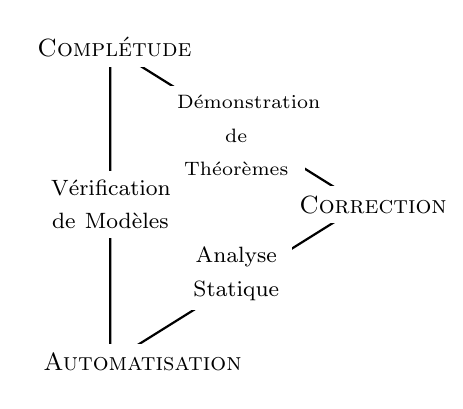
\begin{tikzpicture}[scale=0.8]
    % Dessiner le triangle
    \draw[thick] (0,0) -- (4,2.5) -- (0,5) -- cycle;

    % Placer les sommets avec des bordures bleues
    \node[draw, fill=white, text width=1.7cm, align=center, draw=white] at (0,0) {\small \textsc{Automatisation}};
    \node[draw, fill=white, text width=1.6cm, align=center, draw=white] at (4,2.5) {\small \textsc{Correction}};
    \node[draw, fill=white, text width=1.85cm, align=center, draw=white] at (0,5) {\small \textsc{Complétude}};

    % Placer les étiquettes des arêtes à l'intérieur des arêtes
    \node[fill=white, text width=1.18cm, align=center] at (2,1.4) {\footnotesize Analyse Statique};
    \node[fill=white, text width=1.5cm, align=center] at (0,2.5) {\footnotesize Vérification de Modèles};
    \node[fill=white, text width=1.5cm, align=center] at (2,3.6) {\scriptsize Démonstration de Théorèmes};
\end{tikzpicture}
  \caption{Compromis dans les méthodes formelles.}
  \labfig{formal-methods-trade-offs}
\end{marginfigure}
{\em
\paragraph{Démonstration de théorèmes}

Les prouveurs de théorèmes \sidecite{Nawaz2019} produisent des preuves de correction à l'aide d'outils interactifs, également appelés assistants de preuve, tels que \textsc{Coq} \sidecite{Bertot2004}, \textsc{HOL Light} \sidecite{Harrison2009}, \textsc{Lean} \sidecite{Moura2021}, \textsc{Isabelle} \sidecite{Wenzel2008} et \textsc{Agda} \sidecite{Bove2009}. Les prouveurs de théorèmes sont complets et corrects, mais ne sont pas entièrement automatisés. L'interaction de l'utilisateur est en effet requise pour guider la recherche de preuve. Certaines tentatives visent à automatiser la démonstration de théorèmes \sidecite{Sutcliffe2001} basées sur des stratégies de recherche de preuve où le prouveur recherche automatiquement la preuve. Néanmoins, l'interaction de l'utilisateur est toujours nécessaire lorsque la recherche échoue. Dans cette catégorie de méthodes complètes et correctes, on trouve également des langages de programmation orientés preuve, tels que \textsc{Dafny} \sidecite{Leino2010}, \textsc{F*} \sidecite{Swamy2016}, et \textsc{Why3} \sidecite{Filli_atre2013}.

\paragraph{Vérification de modèles}

Les méthodes formelles basées sur la vérification de modèles \sidecite{Clarke1981,Queille1982} explorent automatiquement l'espace des états d'un modèle de programme pour vérifier si des états indésirables sont atteignables. Les vérificateurs de modèles modernes échangent la terminaison contre l'automatisation et la complétude, car les vérificateurs de modèles ne terminent pas toujours. Lorsque la réponse est \emph{inconnue}, cela signifie que le processus de vérification s'est arrêté sur un dépassement de temps. La propriété peut être satisfaite ou violée, mais le vérificateur de modèles n'a pas pu le déterminer, car l'espace de recherche était trop grand. Cependant, la vérification de modèles est complète car, lorsque le vérificateur indique que la propriété est violée, un contre-exemple est fourni. \sidetextcite{Clarke2004} a appliqué la vérification de modèles pour prouver la correction des programmes ANSI-C.

\paragraph{Exécution symbolique}

L'exécution symbolique \sidecite{Baldoni2018} effectue une exécution abstraite des programmes pour collecter des contraintes sur l'exécution du programme. Pendant la computation abstraite, les variables avec des valeurs inconnues sont représentées symboliquement et propagées à travers le programme. Les contraintes collectées sont ensuite résolues pour vérifier si une assertion est violée ou non. Comme pour la vérification de modèles, l'exécution symbolique échange la correction contre l'automatisation et la complétude. Des outils comme \textsc{KLEE} \sidecite{Cadar2008}, \textsc{BinSec} \sidecite{David2016} et \textsc{PathFinder} \sidecite{Pasareanu2010} sont basés sur l'exécution symbolique.

\paragraph{Analyse statique}

L'analyse statique vérifie le code source du programme à un certain niveau d'abstraction sans interaction utilisateur. Cette abstraction est correcte mais incomplète, ce qui signifie que l'analyse peut signaler des \emph{faux positifs}, c'est-à-dire des avertissements indiquant qu'un programme correct peut être incorrect. Cependant, lorsque l'analyse statique certifie l'absence d'un bogue, le programme est effectivement exempt de bogues. Parmi les méthodes formelles, les techniques d'analyse statique les plus courantes sont basées sur l'\emph{interprétation abstraite}.

\paragraph{Interprétation abstraite}

L'interprétation abstraite \sidecite{Cousot1977} est une théorie générale pour approximer les sémantiques de programmes, développée par Patrick et Radhia Cousot à la fin des années 1970 (voir \sidecite{Cousot2024a} pour une vue historique et \sidecite{Cousot2021} pour une vue d'ensemble). Leur cadre repose sur l'observation que tous les détails computationnels ne sont pas nécessaires pour raisonner sur les propriétés des programmes. Au lieu de cela, la sémantique des programmes peut être approximée par un modèle plus simple et plus abstrait qui facilite le raisonnement automatique.

Au cours de la dernière décennie, les analyses statiques basées sur l'interprétation abstraite sont devenues une partie du cycle de développement des systèmes critiques pour la sécurité. Par exemple, l'analyseur statique \textsc{Astrée} \sidecite{Blanchet2003} est utilisé couramment pour garantir l'absence d'erreurs d'exécution dans les programmes C synchrones embarqués par Airbus.

Nous fournissons une introduction formelle à l'interprétation abstraite dans le \refch{abstract-interpretation}. À la fin de ce chapitre, nous illustrerons les principaux résultats sur un petit langage de programmation idéalisé.

\section*{Utilisation des données d'entrée}

Les erreurs de programmation dans les systèmes logiciels ne conduisent pas toujours à des plantages ou à des erreurs d'exécution. Parfois, des programmes défectueux produisent des résultats plausibles mais erronés, ou des comportements non sûrs. Ces bogues sont difficiles à détecter car ils ne donnent aucun indice clair qu'une erreur s'est produite. Une source potentielle et courante de telles erreurs est la mauvaise utilisation des données d'entrée, c'est-à-dire lorsque la variable d'entrée a un impact inattendu sur le calcul du programme par rapport aux attentes des développeurs.

Un exemple notable est l'article de Reinhart et Rogoff "Growth in a Time of Debt" \sidecite{Reinhart2010}, qui affirmait que la croissance économique est négativement corrélée avec la dette publique. Cet article a été largement cité pour justifier des mesures d'austérité dans le monde entier dans les années qui ont suivi. Cependant, en 2013, \sidetextcite{Herndon2014} a découvert que les auteurs avaient commis une erreur dans leur feuille de calcul Excel, conduisant à une conclusion erronée. L'une des erreurs portait sur l'utilisation incorrecte de la valeur d'entrée relative à la croissance économique de la Norvège en 1964, avec un poids excessif dans le calcul du taux de croissance moyen.

Dans les applications de science des données et d'apprentissage automatique, où les logiciels impliquent de longs pipelines qui filtrent, fusionnent et manipulent des données, les erreurs de programmation provoquant une influence plus ou moins grande des variables d'entrée que prévu sont encore plus probables. Il est donc essentiel d'utiliser des techniques qui renforcent la confiance dans l'utilisation des variables d'entrée pour les applications basées sur les données.

Dans la \arefpart{background}, le \refch{input-data-usage} introduit formellement l'utilisation des données d'entrée, une propriété de programme qui capture l'utilisation \emph{qualitative} des données d'entrée dans un programme, telle que proposée par \textcite{Urban2018}. Nous fournissons une hiérarchie de sémantiques qui capture précisément la propriété d'utilisation des données d'entrée, en abstraisant les détails non nécessaires. Enfin, nous rapportons une sémantique abstraite qui capture les dépendances syntaxiques entre variables de \sidetextcite[][Section 10]{Urban2018}, utilisée pour approximer la propriété d'utilisation des données d'entrée de manière correcte.

\paragraph{Contributions}

Dans le \refch{input-data-usage}, nous étendons la définition originale de l'utilisation des données d'entrée pour capturer des abstractions des valeurs de sortie, de manière similaire à l'interférence abstraite \sidecite{Giacobazzi2018}, en discutant des relations entre ces deux propriétés. Cette extension associe l'interférence abstraite à l'utilisation des données d'entrée, fournissant une définition qui fonctionne de manière native pour les programmes non déterministes sans nécessiter une sémantique de programme spécialisée.

\section*{Propriétés quantitatives}

En général, les propriétés des programmes sont qualitatives : un programme satisfait ou non une propriété. Cela n'est pas toujours suffisant pour capturer la complexité des exigences du monde réel \sidecite{Smith2007}. Par exemple, dans le domaine de la sécurité des programmes, l'une des exigences fondamentales est de protéger la confidentialité des informations sensibles. L'analyse du flux d'information sécurisé se demande si un programme pourrait divulguer des informations sur ses secrets. La non-interférence, qui certifie qu'un programme ne révèle aucune information sur ses secrets, est une approche classique du flux d'informations sécurisé. Cependant, la non-interférence est trop stricte pour de nombreuses applications pratiques. Par exemple, dans un protocole d'élection numérique, les votes individuels doivent rester anonymes, mais le résultat final doit être révélé. Un vérificateur de mot de passe ne doit pas divulguer le mot de passe, mais doit indiquer si le mot de passe est correct. Ces cas représentent des violations délibérées de la non-interférence, nécessaires pour que le programme remplisse son objectif.

Pour répondre à cette limitation, des propriétés quantitatives sont considérées \sidecite{Smith2009}. L'idée clé est d'accepter qu'un programme puisse violer une propriété et de comparer cette violation à un seuil. Les programmes sont classés comme \emph{sûrs} ou \emph{non sûrs} en fonction du degré de violation, ce qui induit une classification des programmes en fonction de leur niveau de sécurité.

Dans le cas de Reinhart et Rogoff, l'erreur n'était pas de savoir si la valeur de la croissance économique de la Norvège avait été utilisée dans le calcul moyen, mais plutôt dans quelle mesure elle avait été utilisée, c'est-à-dire que son impact était beaucoup plus élevé qu'il n'aurait dû l'être. Une analyse quantitative aurait révélé que l'impact de la croissance économique de la Norvège était trop important, permettant aux auteurs de corriger la conclusion erronée.

\subsection*{Vérification quantitative des propriétés extensionnelles}

\marginnote{\refch{quantitative-input-data-usage} et \refch{showcase} dans la \arefpart{extensional} sont basés sur les travaux publiés au NASA Formal Methods Symposium (NFM) 2024 \cite{Mazzucato2024b}.}
\marginnote{\formatmargincitation{Mazzucato2024b}}

Dans la première partie de cette thèse, nous proposons des techniques d'analyse statique basées sur la sémantique pour quantifier l'impact des variables d'entrée sur la computation des programmes. Dans le \refch{quantitative-input-data-usage}, nous introduisons un nouveau cadre formel basé sur l'interprétation abstraite pour raisonner sur les propriétés quantitatives de l'utilisation des données d'entrée. Ce cadre permet d'identifier les variables ayant un impact disproportionné, certifiant ainsi le comportement prévu ou révélant d'éventuelles failles en comparant les attentes des développeurs avec les résultats réels. Nous caractérisons l'impact d'une variable d'entrée par une notion de dépendance entre les variables et les résultats du programme. Notre cadre est paramétrique en fonction de la définition d'impact choisie.

Nous introduisons une analyse statique rétrograde basée sur l'interprétation abstraite, paramétrique en fonction de la définition d'impact, qui infère une sur-approximation correcte de l'impact des variables d'entrée. Cette approche permet aux utilisateurs finaux de choisir l'impact qui correspond à leurs besoins, garantissant une analyse ciblée et personnalisable.

Le \refch{showcase} démontre les applications potentielles du cadre quantitatif en évaluant notre outil d'analyse statique, \impatto\sidenote{\label{intro:impatto}\impattourl}, sur six cas d'utilisation.

\marginnote{\refch{quantitative-fairness} et \refch{evaluation-on-neural-networks} dans la \arefpart{extensional} sont basés sur les travaux publiés au 28e Symposium d'analyse statique (SAS) 2021 \cite{Mazzucato2021}.}
\marginnote{\formatmargincitation{Mazzucato2021}}

Dans le \refch{quantitative-fairness}, nous étendons la propriété d'utilisation quantitative des données d'entrée aux réseaux neuronaux. Nous proposons deux quantificateurs d'impact pour les réseaux neuronaux, en répondant aux défis découlant de l'espace d'entrée hautement non linéaire et en mesurant l'équité des caractéristiques d'entrée. Nous affinons l'analyse rétrograde pour exploiter les calculs parallèles afin d'améliorer les performances, en utilisant une combinaison d'analyse directe et rétrograde. La passe directe réduit l'explosion combinatoire de l'analyse rétrograde en partitionnant l'espace d'entrée en sous-régions pour une parallélisation plus facile. Le \refch{evaluation-on-neural-networks} montre l'efficacité de notre approche sur les réseaux neuronaux, prouvant que notre méthode peut identifier les caractéristiques d'entrée ayant un impact disproportionné sur la sortie du réseau ou quantifier l'équité des réseaux neuronaux.

\paragraph{Contributions}
Les contributions suivantes font partie de la \arefpart{extensional}, composée des \cref{ch:quantitative-input-data-usage,ch:showcase,ch:quantitative-fairness,ch:evaluation-on-neural-networks} :

\begin{itemize}
  \item Dans le \refch{quantitative-input-data-usage}, nous développons un cadre théorique par interprétation abstraite pour quantifier l'impact des variables d'entrée en considérant trois nouveaux quantificateurs d'impact.
  \item Dans le \refch{quantitative-input-data-usage}, nous présentons notre analyse statique et une possible implémentation abstraite des instances d'impact.
  \item Dans le \refch{showcase}, notre outil \impatto{} illustre notre approche sur un ensemble de six programmes démonstratifs.
  \item Un artefact de \impatto{} comprenant le code source, la documentation et les benchmarks d'évaluation est disponible sur Zenodo\sidenote{\impattozenodo}.
  \item Dans le \refch{quantitative-fairness}, nous présentons deux nouveaux quantificateurs d'impact pour les réseaux neuronaux.
  \item Dans le \refch{quantitative-fairness}, nous proposons une analyse rétrograde améliorée qui exploite les calculs parallèles et atteint une meilleure précision en combinant les domaines abstraits.
  \item Dans le \refch{evaluation-on-neural-networks}, nous avons étendu les outils \impatto{} et \libra\sidenote{\libraurl} pour évaluer notre analyse quantitative sur les réseaux neuronaux.
  \item Un artefact étendant \libra{} avec l'évaluation quantitative de l'équité est disponible sur Zenodo\sidenote{\librazenodo}.
\end{itemize}

\subsection*{Vérification quantitative des propriétés intentionnelles}

\marginnote{\arefpart{intensional} est basée sur les travaux publiés au 31e Symposium d'analyse statique (SAS) 2024 \cite{Mazzucato2024c}.}
\marginnote{\formatmargincitation{Mazzucato2024c}}

La \arefpart{intensional} se concentre sur la vérification quantitative des propriétés intentionnelles, c'est-à-dire des propriétés qui dépendent du comportement interne du programme, comme le nombre d'itérations d'une boucle. Cette partie est divisée en deux chapitres : le premier présente la nouvelle analyse du temps d'exécution quantitative, et le second montre l'évaluation expérimentale.

Dans le \refch{quantitative-static-timing-analysis}, nous considérons le nombre d'itérations du programme comme le résultat du programme, capturant l'impact des variables d'entrée sur le nombre global d'itérations. Nous sommes donc capables de découvrir des erreurs de programmation affectant les itérations qui peuvent dégrader les performances ou introduire des vulnérabilités de sécurité sans erreurs fonctionnelles. Par exemple, les impacts inattendus des données d'entrée sur le temps d'exécution pourraient révéler des informations sensibles \sidecite{Wong2005}, posant ainsi des menaces à la sécurité. Même les programmes cryptographiques sont vulnérables aux attaques par canaux auxiliaires temporels, en fonction des choix d'implémentation. \sidetextcite{Kocher1996} a démontré que les algorithmes cryptographiques à clé publique, tels que RSA, sont susceptibles d'être attaqués via des canaux auxiliaires temporels, potentiellement exposant les clés secrètes.

Pour l'optimisation des performances, identifier les variables d'entrée qui affectent de manière significative les itérations de boucle aide les développeurs à se concentrer sur les segments de code critiques \sidecite{Omar2017}. Par conséquent, comprendre l'impact des variables d'entrée sur le temps d'exécution est primordial. Dans cette seconde partie de la thèse, nous nous concentrons sur la quantification de l'impact des variables d'entrée sur les itérations de boucle comme indicateur du comportement temporel.

Nous exploitons une analyse des bornes globales des boucles pour dériver une sur-approximation des bornes globales des boucles, en encodant la quantification de l'impact des variables d'entrée comme un problème de programmation linéaire. Notre approche combine des informations syntaxiques et sémantiques : générer des invariants sous forme de contraintes linéaires pour la précision et combiner une analyse des bornes globales avec une analyse de dépendance syntaxique \sidecite[][Section 10]{Urban2018} pour l'évolutivité.

Dans le \refch{sas24-eval}, nous présentons \timesec\sidenote{\timesecurl}, un outil implémentant notre analyse du temps d'exécution quantitative. Nous démontrons son efficacité dans la bibliothèque cryptographique \bignum{} d'Amazon Web Services\sidenote{\bignumurl}, en certifiant son immunité contre les attaques par canaux auxiliaires temporels en montrant l'absence d'impact des variables d'entrée sur les itérations de boucle. De plus, nous évaluons \timesec{} sur des programmes issus de \svcomp\sidenote{\svcompurl}, une suite de tests conçue pour les outils de vérification de logiciels.

\paragraph{Contributions}

Les contributions suivantes appartiennent à la \arefpart{intensional} :

\begin{itemize}
  \item Dans le \refch{quantitative-static-timing-analysis}, nous proposons une analyse statique utilisant un domaine abstrait de contraintes linéaires, une analyse des bornes globales des boucles et un encodage en programmation linéaire pour quantifier l'impact des variables d'entrée sur les itérations de boucle.
  \item Dans le \refch{sas24-eval}, nous présentons \timesec\sidenote{\timesecurl}, un outil implémentant notre analyse du temps d'exécution quantitative, et nous l'évaluons sur la bibliothèque cryptographique \bignum\sidenote{\bignumurl} ainsi que sur les programmes de \svcomp\sidenote{\svcompurl}.
  \item Un artefact de \timesec{} comprenant le code source et les benchmarks d'évaluation est disponible sur Zenodo\sidenote{\timeseczenodo}.
\end{itemize}

\frenchdiv

Les travaux connexes sont discutés à la fin de chaque chapitre, fournissant une vue d'ensemble complète de la littérature pertinente. À la fin de la thèse, dans la \arefpart{conclusion}, nous concluons avec un résumé et des perspectives sur les futures directions de recherche.
}
